\chapter{Datenerfassung}

In Abbildung \ref{fig:versuchsaufbau} ist der Versuchsaufbau zur Datenerfassung 
zu sehen. Alle wichtigen Bestandteile sind nummeriert. Es folgt eine kurze Benennung
aller vorhandenen und notwendigen Teile:\\
1: Schraubstock Backen\\
2: Demonstratorbauteil\\
3: Scannerhalterung\\
4: Scanner LLT 30x0-25\\
5: Verschiebungsmesser\\
6: Schraubstock mit Kraftmesser\\
7: Laserlinie (Lila)\\

Der Scanner ist an dem Werkzeugkopf einer CNC-Fräse befestigt und wird 
in Richtung der X und Y Achse verschoben. So kann von dem kompletten Bauteil ein
Daten-Set mithilfe des Scanners aufgenommen werden.

\section{Zusätzliche Messinstrumente}

Zusätzlich zu dem Scanner werden noch mit weiteren Messinstrumente Daten erfasst.
In Abbildung \ref{fig:versuchsaufbau} unter der Nummer 5 ist ein mechanischer 
Verschiebungsmesser zu sehen. Dieser misst die Verschiebung der Backen des 
Schraubstocks. Der Schraubstock misst zusätzlich mit viel Kraft die Backen 
aufeinander pressen.

\begin{figure}[H]
    \centering
    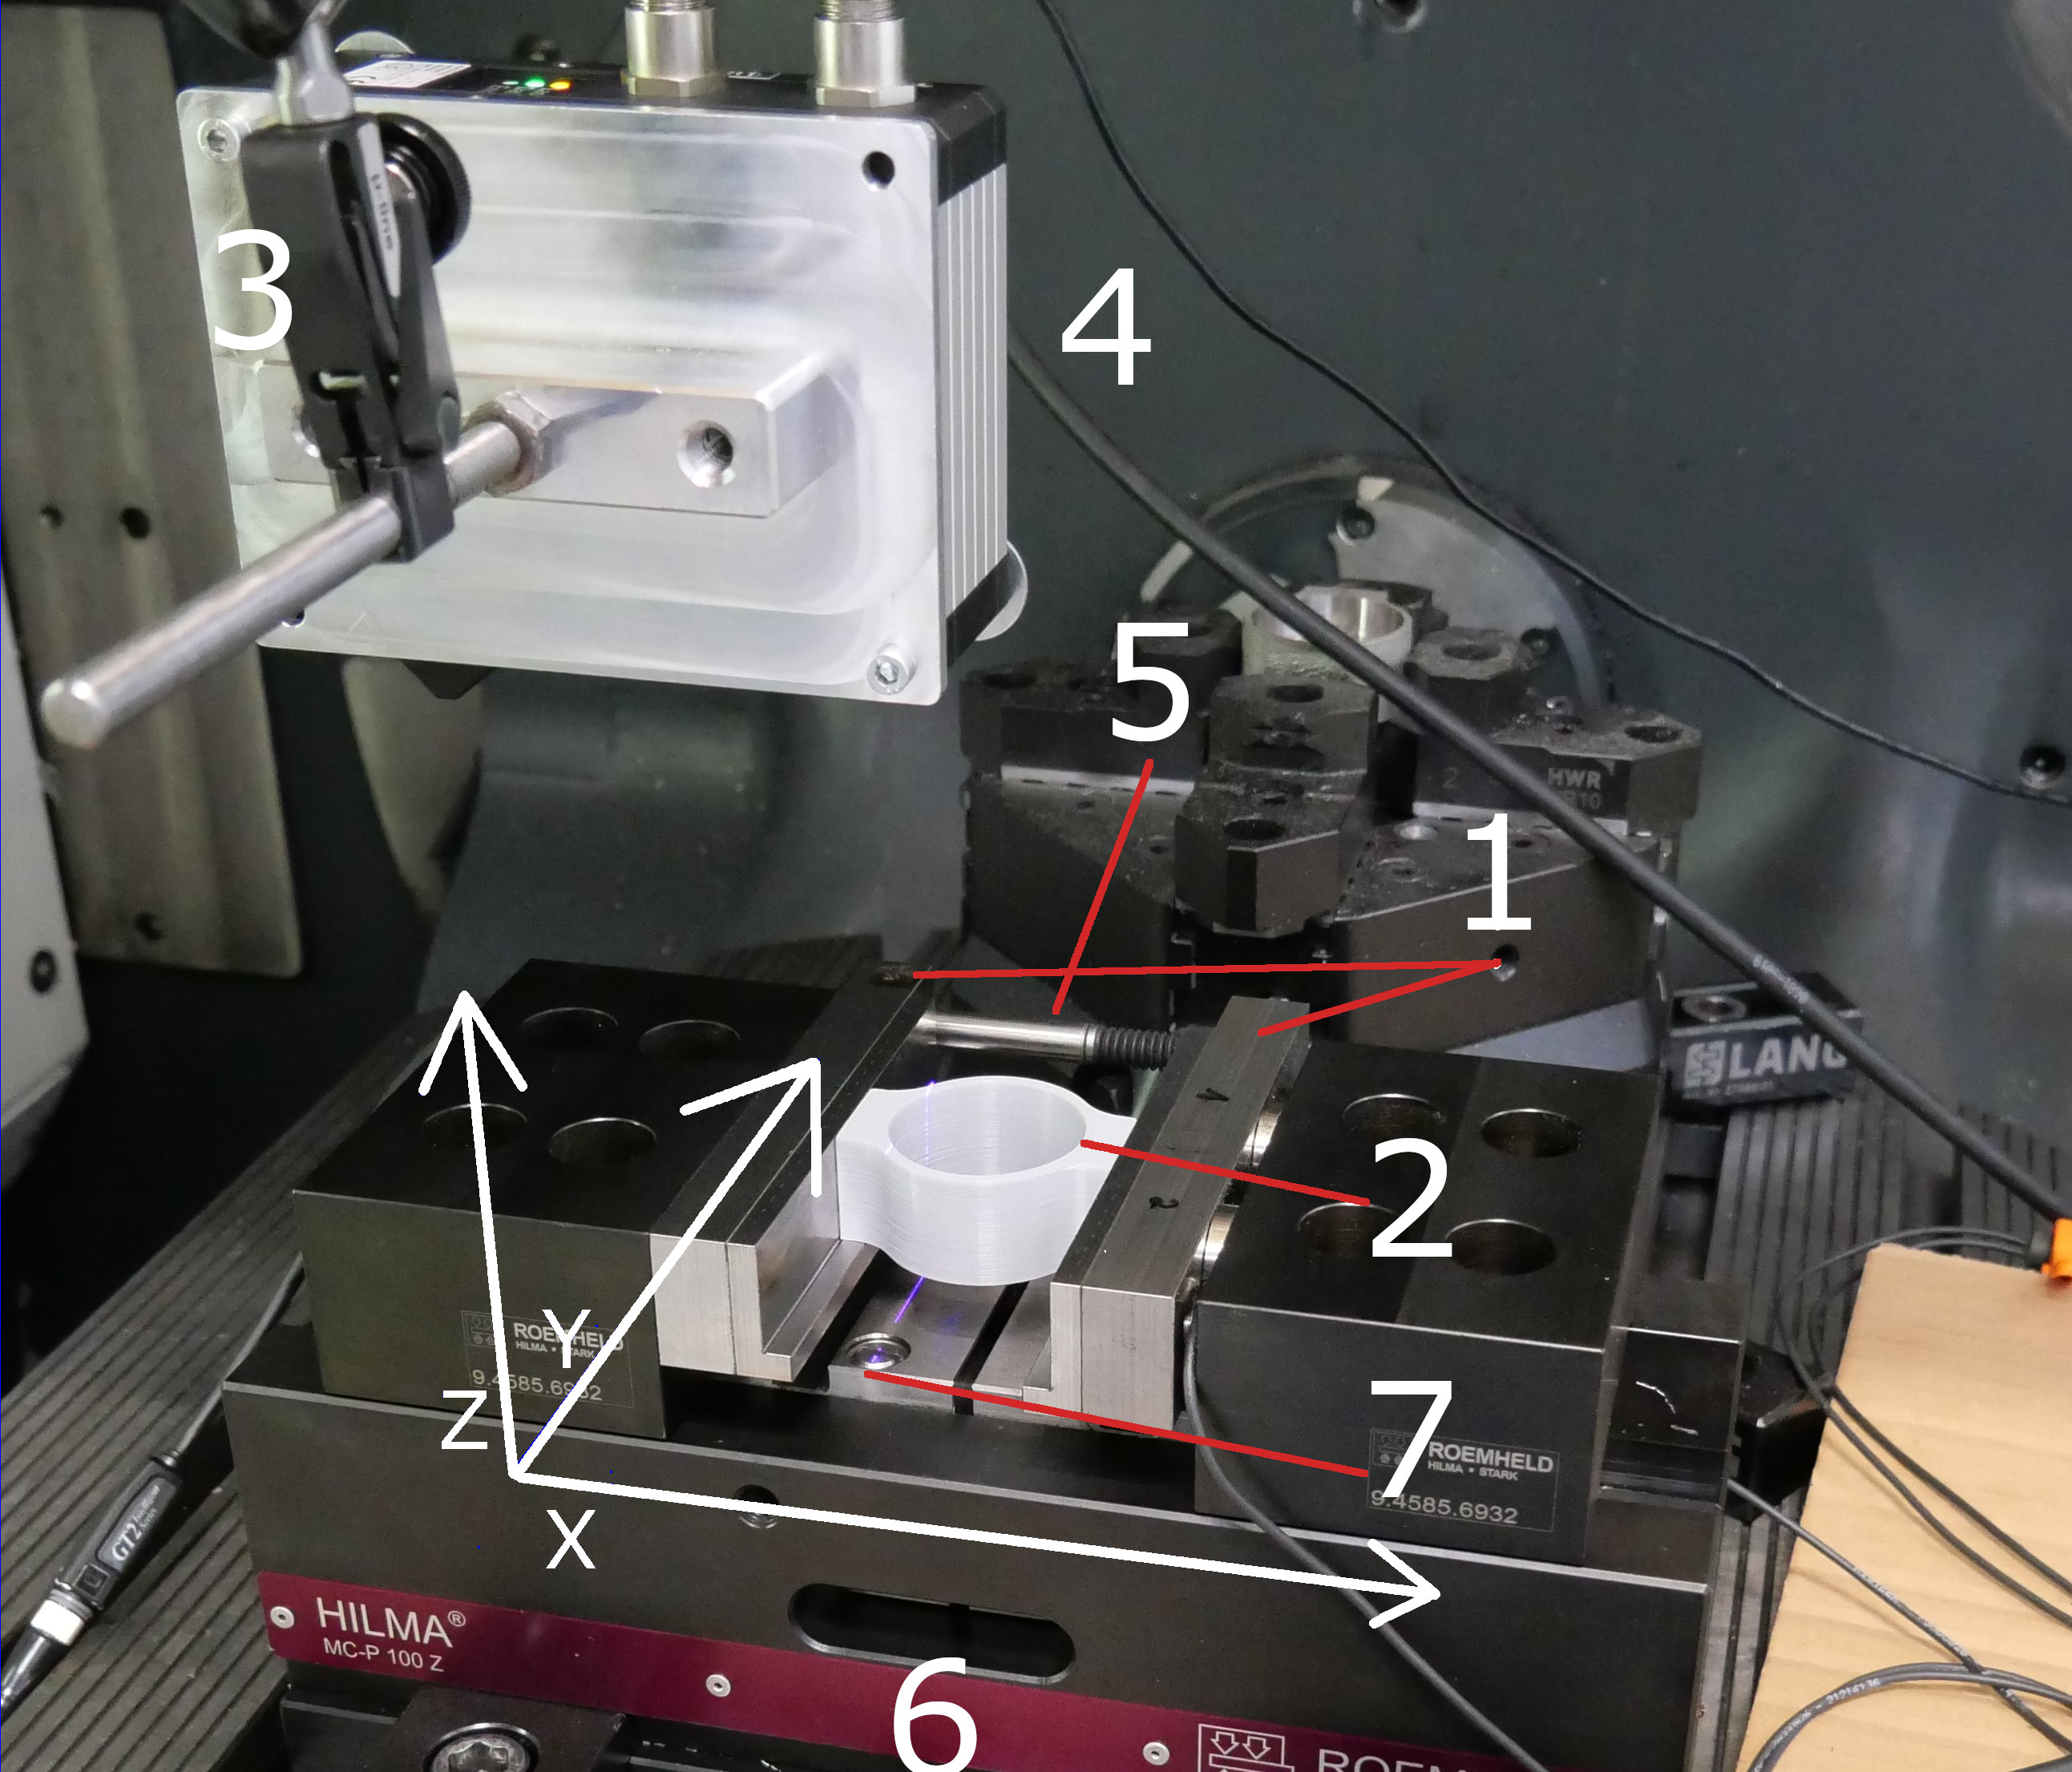
\includegraphics[width=0.6\textwidth]{images/versuchsaufbau_foto.png.JPG}
    \caption{Versuchsaufbau}
    \label{fig:versuchsaufbau}
\end{figure}

Hierzu wird die piezoelektrische Kraftmesstechnik verwendet.
Bei Krafteinwirkung auf Piezokristalle (z. B. Quarz, Bariumtitanat, BaTiO3) 
werden im Kristallgitter negative gegen positive Gitterpunkte
verschoben, sodass an den Kristalloberflächen
Ladungsunterschiede Q als Funktion der Kraft F
gemessen werden.
Piezoelektrische Kraftaufnehmer sind mechanisch sehr steif, 
sie erfordern Ladungsverstärker
zur Messsignalverarbeitung und sind hauptsächlich zur Messung dynamischer Vorgänge
mit einer kleineren Frequenz als 1 Hz geeignet. \cite{Czichos.2020}. 
Diese Kraftmesstechnik ist 
für unseren Einsatzzweck gut geeignet da sie eine hohe Empfindlichkeit bietet 
und in vielfältigen Formen und Größen hergestellt werden kann. Zur Aufbereitung 
der Ladung, die der piezoelektrische Sensor, liefert wurde ein Ladungsverstärker 
eingesetzt.\cite{Schwartz.2006}

\section{Demonstratorbauteil} \label{demo_Bauteil}

Für die Validierung des Verfahrens wurde ein Demonstratorbauteil ausgewählt.
Dieses ist im Versuchsaufbau unter zwei zu sehen. Dieses Bauteil wurde ausgewählt 
weil, die Deformation an der äußeren und inneren Bauteilgeometrie gemessen werden kann.
Zusätzlich wird durch den dünnen Rand gewährleistet das auch bei einem Metallteil 
eine Deformation stattfindet.
Das Demonstratorbauteil existierte für die Datenerfassung in mehrere Versionen.
Um Werkstoffe vergleichen zu können, liegt das Bauteil einmal als FDM Druck aus PLA vor 
und einmal als additiv gefertigtes Metallteil.
Das Metallteil wurde mit drei verschiedenen Stützstruktur vermessen, um die Auswirkung 
der Stützstruktur auf die Deformation zu erkennen. In Abbildung \ref{fig:demofdm} ist 
das Demonstratorbauteil zu sehen, dass per FDM gedruckt wurde.

\begin{figure}[H]
    \centering
    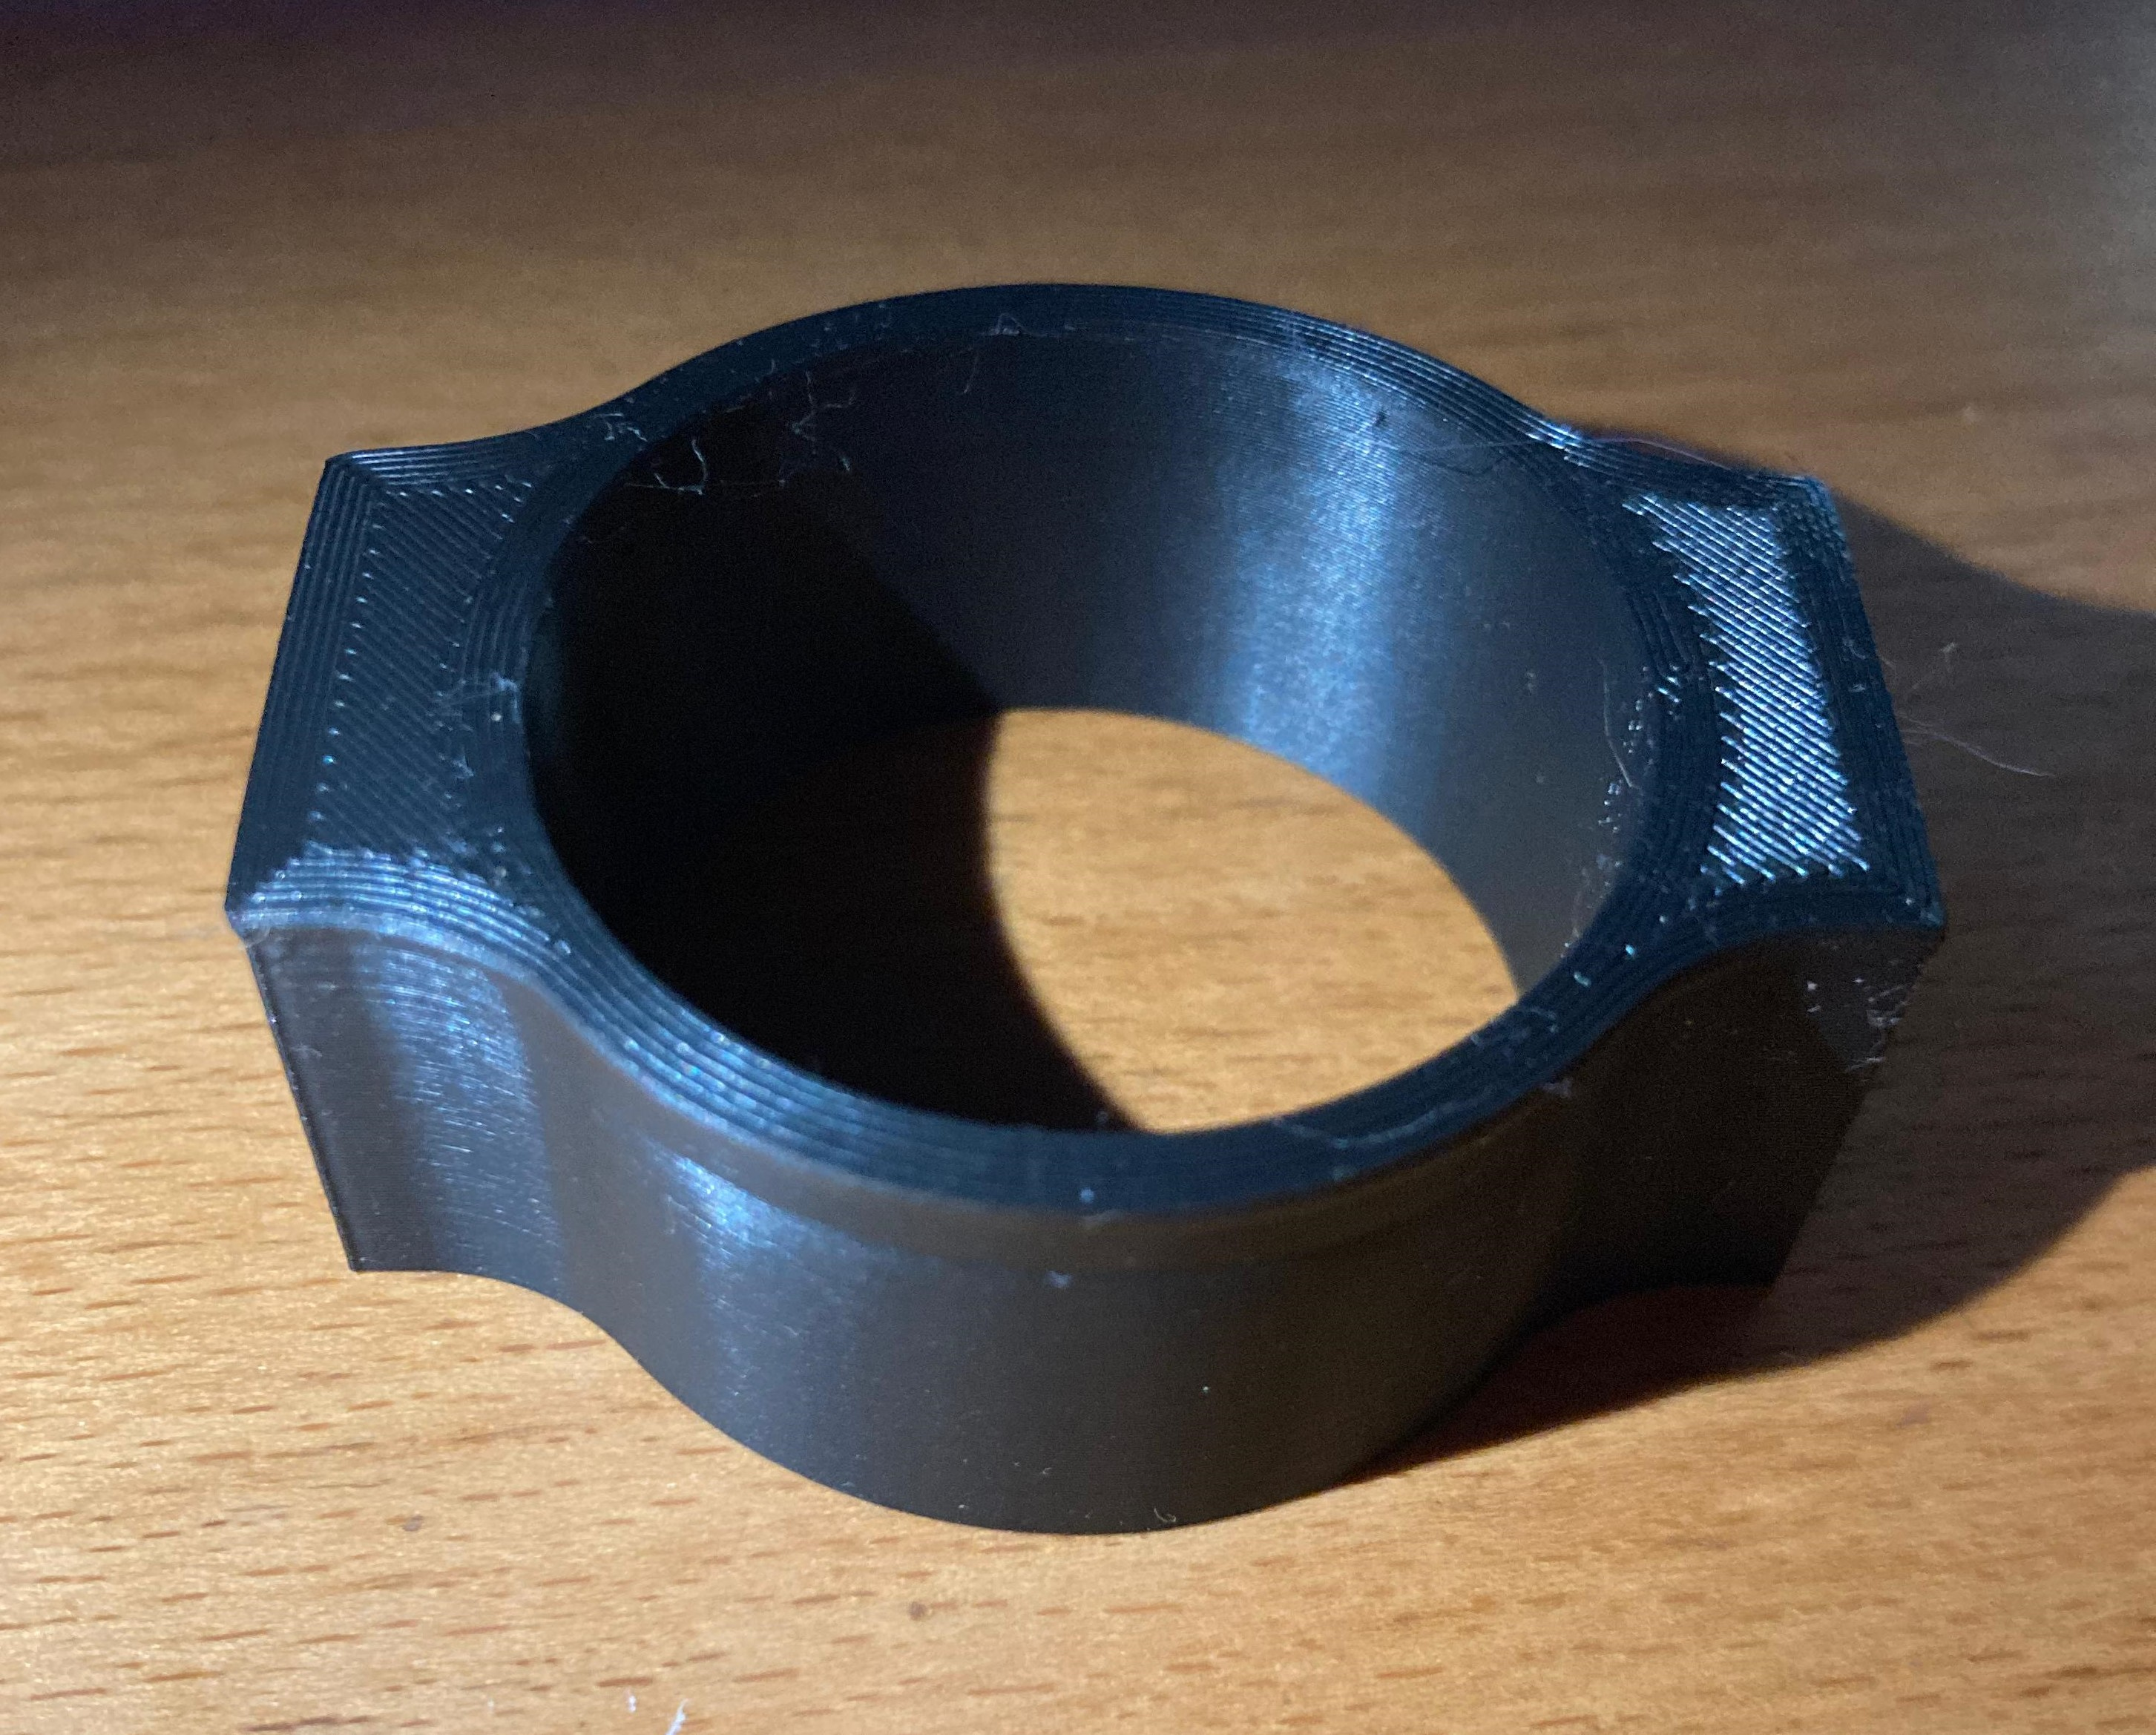
\includegraphics[width=0.6\textwidth]{images/demo_fdm.jpg}
    \caption{FDM gedrucktes Demonstratorbauteil.}
    \label{fig:demofdm}
\end{figure}
